\chapter{Android}\label{sec:Android}
This chapter will provide information about Android and Wear 2.0 technology. Why it was developed and what are the differences between previous version and other wear technologies.

\medskip

Android is a Linux based operating system for mobile and wear devices developed by Google. The main selling point of this system is that it's open-source project, meaning that everyone can access the code and modify it as they wish. Android was mainly developer for mobile phones but since that time it moved beyond that by being implemented to all kinds of wear devices, tablets, televisions and even refrigerators or cameras.\cite{WIGA}

\section{Android system structure}\label{sec:AndroidSystemStructure}
Android is created as a stack, meaning there are functional modules stack on top of each other from Linux core over native libraries to applications as shown in \fref{fig6}. Android maintains complete software stacks to enable device creators to run and modify Android for their specific hardware. To support these modifications and testing every release has multiple "code lines" to separate stable versions from experimental work.\cite{AOSP}

\begin{figure}[H]
	\begin{centering}
		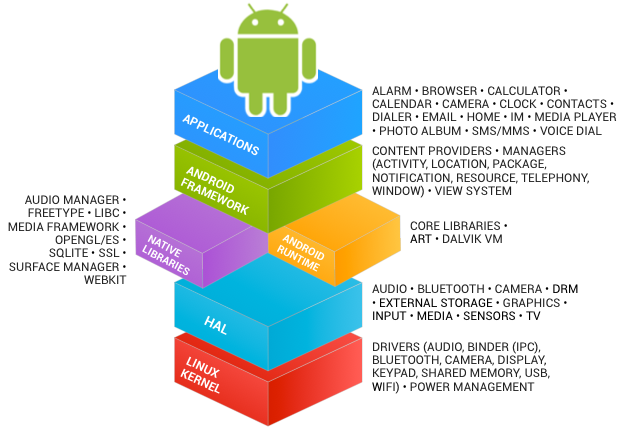
\includegraphics[width=0.6\textwidth]{img/android_stack}
		\par\end{centering}
	\caption{Android stack (source: \cite{AOSP})\label{fig:AndroidStack}}
	\label{fig6}
\end{figure}

There are multiple versions of Android system at this time and every single one has it's own version, code name and API level. Version codes are number identifications of a specific system version. Highest levels of these numbers are grouped into code names that are ordered alphabetically. As an example versions 8.0.0 and 8.1.0 have the same code name called Oreo. Finally API level is number identification for compatibility of specific application and it will be compared to API level of device Android system.\cite{AOSP}\cite{AD}

Android security...

\section{Wear technologies}\label{sec:WearTechnologies}
Interactive wearable, as an example smart watches, is a new part of mobile computers. Wear devices are categorically different from phones or tables in term of usage, design and user interfaces (UI). According to the app design guidelines by major vendors, users interact with wearable devices frequently throughout daily use. Each interaction is short, often less than 10 seconds, and is dedicated to simple tasks.\cite{UtCoAWO}

\subsection{Android Wear}\label{sec:AndroidWear}

\section{Other wear technologies}\label{sec:OtherWearTechnologies}
Pebble, Apple, Microsoft ...